\documentclass[nobib]{tufte-handout}

%\\geometry{showframe}% for debugging purposes -- displays the margins

\newcommand{\bra}[1]{\left(#1\right)}
\usepackage{amssymb}
\usepackage{hyperref}
\usepackage[activate={true,nocompatibility},final,tracking=true,kerning=true,spacing=true,factor=1100,stretch=10,shrink=10]{microtype}
\usepackage{color}
\usepackage{steinmetz}
% Fixes captions and images being cut off
\usepackage{marginfix}
\usepackage{array}
\usepackage{tikz}
\usepackage{amsmath,amsthm}
\usetikzlibrary{shapes}
\usetikzlibrary{positioning}
\usepackage{listings}
\usepackage{caption}
\usepackage{circuitikz}
\DeclareCaptionFont{white}{\color{white}}
\DeclareCaptionFormat{listing}{\colorbox{gray}{\parbox{\textwidth}{#1#2#3}}}
\captionsetup[lstlisting]{format=listing,labelfont=white,textfont=white}

% Set up the images/graphics package
\usepackage{graphicx}
\setkeys{Gin}{width=\linewidth,totalheight=\textheight,keepaspectratio}
\graphicspath{{.}}

\title{Notes for ECE 36200 - Microprocessor Systems and Interfacing}
\author[Shubham Saluja Kumar Agarwal]{Shubham Saluja Kumar Agarwal}
\date{\today}  % if the \date{} command is left out, the current date will be used

\usepackage{pgfplots}
% The following package makes prettier tables.  We're all about the bling!
\usepackage{booktabs}

% The units package provides nice, non-stacked fractions and better spacing
% for units.
\usepackage{units}

% The fancyvrb package lets us customize the formatting of verbatim
% environments.  We use a slightly smaller font.
\usepackage{fancyvrb}
\fvset{fontsize=\normalsize}

% Small sections of multiple columns
\usepackage{multicol}

% For finite state machines 
\usetikzlibrary{automata} % Import library for drawing automata
\usetikzlibrary{positioning} % ...positioning nodes
\usetikzlibrary{arrows} % ...customizing arrows
\tikzset{node distance=2.5cm, % Minimum distance between two nodes. Change if necessary.
    every state/.style={ % Sets the properties for each state
    semithick,
    fill=gray!10},
    initial text={}, % No label on start arrow
    double distance=2pt, % Adjust appearance of accept states
    every edge/.style={ % Sets the properties for each transition
    draw,
    ->,>=stealth', % Makes edges directed with bold arrowheads
    auto,
    semithick}}
\let\epsilon\varepsilon

% These commands are used to pretty-print LaTeX commands
\newcommand{\doccmd}[1]{\texttt{\textbackslash#1}}% command name -- adds backslash automatically
\newcommand{\docopt}[1]{\ensuremath{\langle}\textrm{\textit{#1}}\ensuremath{\rangle}}% optional command argument
\newcommand{\docarg}[1]{\textrm{\textit{#1}}}% (required) command argument
\newenvironment{docspec}{\begin{quote}\noindent}{\end{quote}}% command specification environment
\newcommand{\docenv}[1]{\textsf{#1}}% environment name
\newcommand{\docpkg}[1]{\texttt{#1}}% package name
\newcommand{\doccls}[1]{\texttt{#1}}% document class name
\newcommand{\docclsopt}[1]{\texttt{#1}}% document class option name

% Define a custom command for definitions and biconditional
\newcommand{\defn}[2]{\noindent\textbf{#1}:\ #2}
\let\biconditional\leftrightarrow

\begin{document}

\maketitle

\begin{abstract}
    These are lecture notes for spring 2024 ECE 36200 at Purdue as taught by Professor Younghyun Kim. Modify, use, and distribute as you please.
\end{abstract}

\tableofcontents

\newpage
\section{GPIO}

The idea behind a GPIO pin is the fact that it can do basically anything, due
to which it is called General Purpose.\\

The structure of a GPIO pin is the following:\\
\begin{center}
    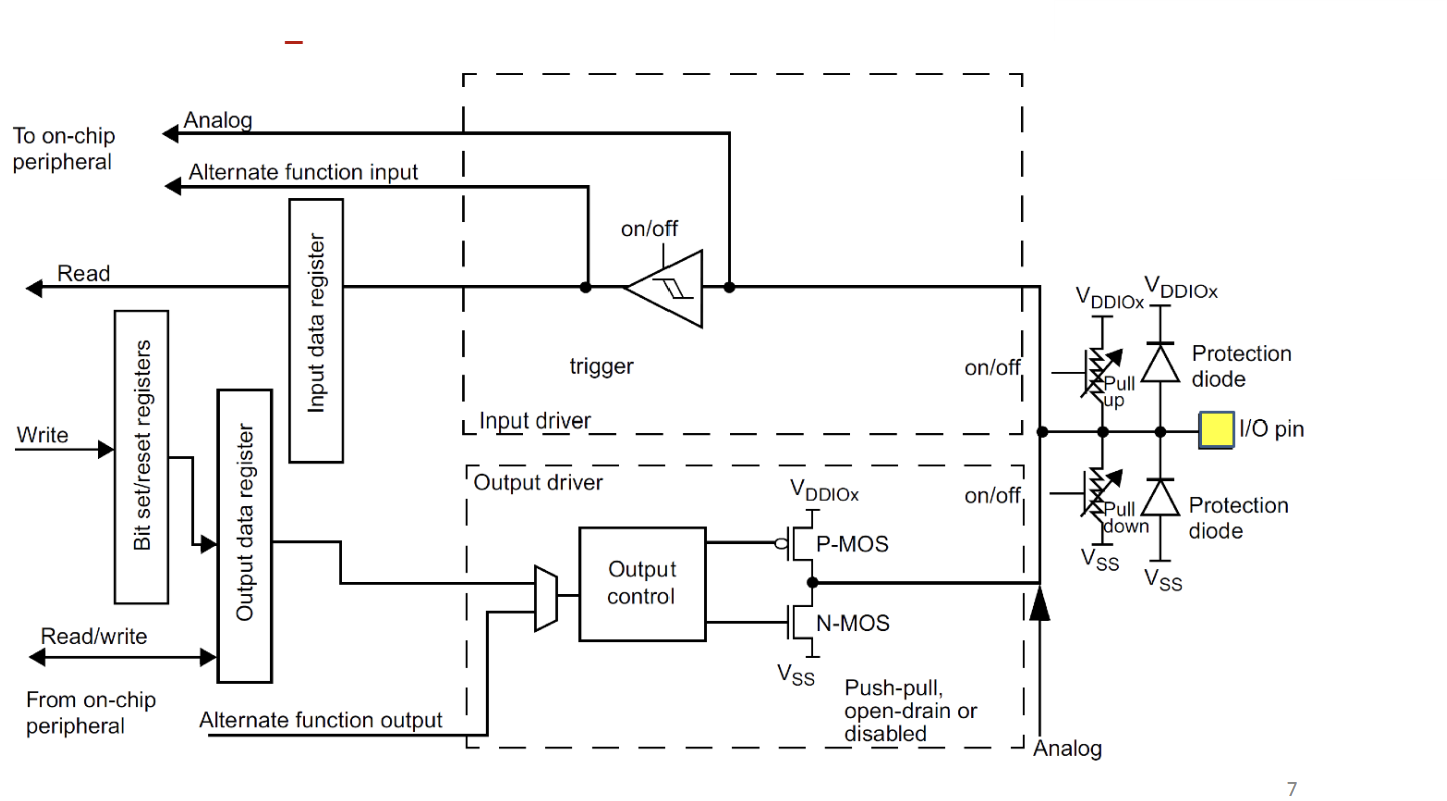
\includegraphics[width = 300px]{images/gpio_circuitry.png}
\end{center}

This circuit can be broken down into two parts - Output control and Input
Control.

\subsection{Output Control}

Output Control, can be written to by bit set/reset registers, or by read/write
operations.\\ Bit set/reset registers are registers within the microcontroller
that connect to specific pins on the board. When the program writes to these
registers, depending on which operation was executed, it will make the Output
Data Register output a high or low bit (set and reset respectively).\\ On the
other hand, read/write operations directly write in the bit they want written
to the pin, without the use of BSRRs.\\

Once one of these operations is executed, the ODR sends connects to a
multiplexer, which, in turn, connects to the output control. This will, in fact
act as an inverter, as it will output a 0 if the input is 1, and output a 1 if
the input is 0.\\

The output control connects to a pair of transistors which can be set to two
modes aside from disabled - push-pull and open-drain.\\ When the output control
is set to push-pull, it is connected to two transistors in an inverting setup.
This allows it to flip the previously inverted values once again, thus allowing
the output to be what was written in to the pin.\\ When the output is
open-drain, the PMOS transistor is left floating, while the NMOS transistor is
connected to a pull-up resistor. So, when the output control writes a 0, the
NMOS remains open, and is pulled up by the resistor. Otherwise, the NMOS closes
and connects the output to ground.\\ The output is then set to the values
defined by the previous section.

The speed at which the output value changes is known as slew rate, that is:

\begin{equation*}
    Slew_{Rate} = \max(\frac{\Delta V}{\Delta t})
\end{equation*}

\subsection{Input Control}
Input Control consists of a pull-up or pull-down resistor, and a Schmitt
Trigger. The pull-up or pull-down resistor prevents the value being read from
the IO pin from ever floating. The user must decide which of the two resistors
they wish to enable.\\ The Schmitt Trigger acts as a buffer. It's purpose is to
minimize the fluctuations of the input pin, as well as forcing the value to be
a high or a low (like a comparator). It has two voltage values, which we can
call $V_{high}$ and $V_{low}$. When the input to the diode is greater than
$V_{high}$, it toggles from low to high. When it is lower than $V_{low}$, it
toggles from high to low. If this were not present, if the voltage were to
fluctuate a lot around the toggle value, the voltage would keep on toggling
between high and low, which would not be ideal.\\

\subsection{Things to consider}

A buffer, like the Schmitt Trigger, needs to have well defined inputs, that is,
they should not be floating. To do this, there must be pull-up or pull-down
resistors connected to the inputs, of values lower than the internal resistance
of the buffer itself. Whether it is pull-up or pull-down is defined by what the
input of the buffer is connected to by default. If it is connected to ground by
default, then it needs a pull-up resistor, otherwise, it needs a pull-down
resistor.\\ High resistance means slow adjustments of voltage, and are thus
considered weak pull up or down resistors.

\subsection{GPIO control}
The functionality of GPIO pins is defined by writing different values to the
GPIO control registers.\\ Note: to write something to a single bit in a
register, we use "|=" for high, and "!(\&=)" for low.

\section{Interrupts}
Interrupts are called by the peripherals when a predefined even occurs, this
can be a timer overflowing, or a pin receiving data, among others.\\ There are
three main parameters on interrupts: ISR, EN, Pri.

\begin{itemize}
    \item ISR: Index of the routine, the lower the value, the higher the priority of the
          interrupt.
    \item EN: marks whether the interrupt is enabled, if it is not, it cannot be raised,
          and should thus not be considered.
    \item Pri: It is another method of indicating priority, and can override the
          priorities defined by the ISR.
\end{itemize}

Now that we know all these, we can understand how these behave.\\ Let us say
that the program is running in main and an interrupt is called. It will be
marked as pending. The program will check if the priority of the pending
interrupt is higher than the current running program (if it is main, then it
will always be higher). If it is, the current state will be saved, and the
program will execute the interrupt. This process is constantly executed, so, if
higher priority interrupts are called during an interrupt, it will save once
again, and address that interrupt again. If the interrupt being called is of
lower priority than what is running at the given moment, it is marked as
pending. When the interrupt finishes running, it will head to the interrupt
with the highest priority that is pending. Once all the pending interrupts are
addressed, the program returns to main.\\

\section{Timers}
Timers allow the microcontroller to execute things periodically.\\ Every clock
cycle the program checks whether the value stored in the hardware counter is 0.
If not, the value stored is decrease by 1, otherwise, it copies the reload
value into the counter and raises an interrupt if enabled.\\ So, the interrupt
is called every $(reload_{value}+1)*clock_{period}$.\\ There also exist more
general timers, which have an additional parameter, the prescaler, which
changes the equation to:
\begin{equation*}
    reload_{value} = \frac{interrupt_{interval}}{clock_{period}*(prescaler + 1)}
\end{equation*}
as opposed to the equation for the system timer:
\begin{equation*}
    reload_{value} = \frac{interrupt_{interval}}{clock_{period}}-1
\end{equation*}
\section{DMA}
DMA optimizes data copying/data movement. Normal copying requires the
peripheral to write the data to the CPU, and then the CPU writes the data to
the destination.\\ On the other hand DMA directly copies the data to the
destination, without ever interacting with the CPU.\\ There are two kinds of
DMA:\\
\begin{itemize}
    \item Flow-Through: Connects to the DMA controller, and is then sent over. This is
          slower than fly-by, however, it simplifies the wiring. Used as long as the
          requirements for speed are not too stringent. It is also more convenient for
          cases where the destination and origin registers are of different sizes.
    \item Fly-By: Connects all the wires directly, making the space utilization worse,
          but speeding up the transfer speed considerably. Useful when read and write
          operations are executed in the same cycle.
\end{itemize}
\section{DAC}
If we base
\begin{equation*}
    DAC_{output} = V_{ref} \times \frac{Digital_{Value}}{2^N}
\end{equation*}
With default N = 12.\\
Digital Value is:
\begin{equation*}
    \sum_{i=0}^{N-1}2^{i}\times DAC_{bit}[i]
\end{equation*}

\end{document}

